\documentclass[tikz,border=10pt]{standalone}
\usepackage{tikz}
\usetikzlibrary{shapes.geometric, arrows.meta, positioning, calc}
\definecolor{cindigo}{RGB}{79, 70, 229}
\definecolor{cgold}{RGB}{217, 119, 6}
\definecolor{cambergold}{RGB}{254, 243, 199}
\begin{document}
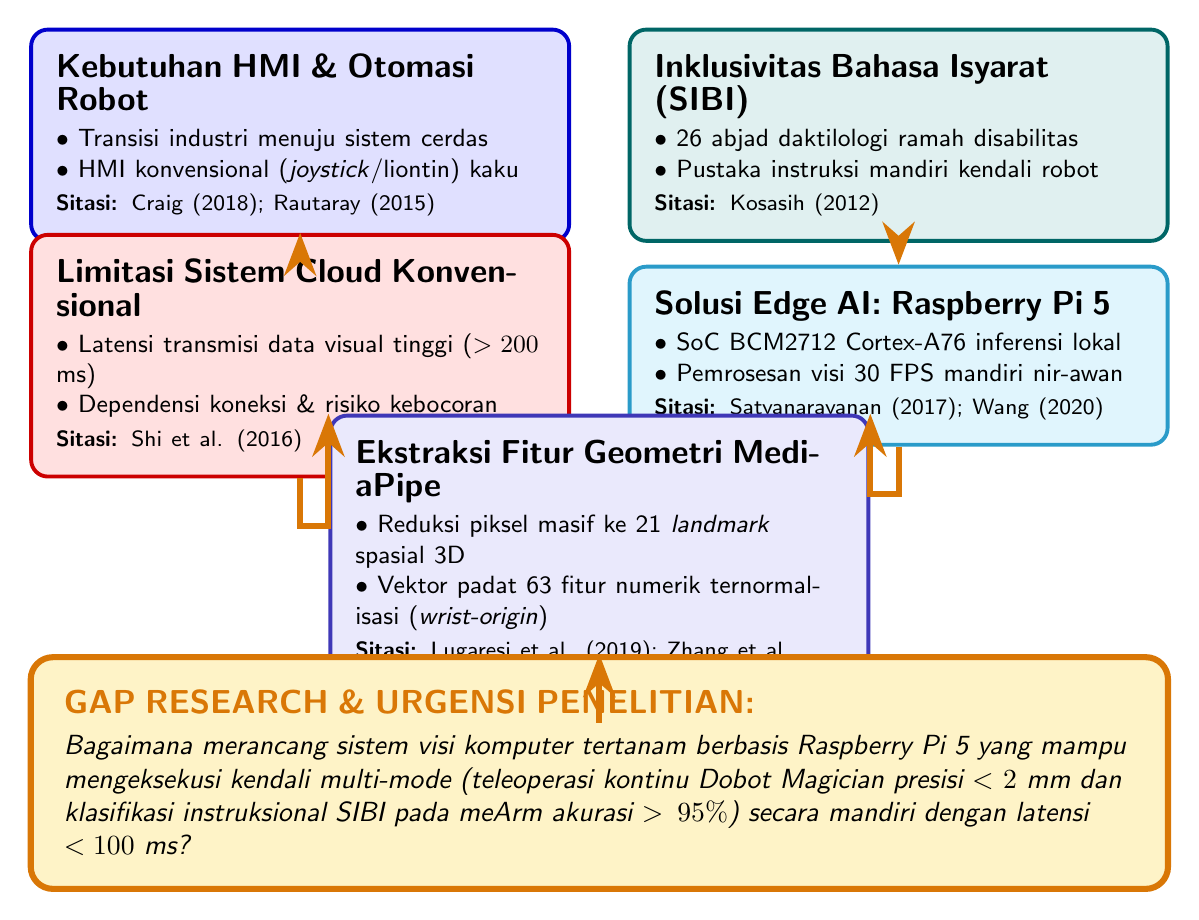
\begin{tikzpicture}[
    font=\sffamily,
    box/.style={
        rectangle, draw=#1!80!black, rounded corners=6pt, fill=#1!12,
        line width=1.4pt, inner sep=9pt, text width=6.2cm, align=left
    },
    gapbox/.style={
        rectangle, draw=cgold, rounded corners=8pt, fill=cambergold,
        line width=2.2pt, inner sep=12pt, text width=13.6cm, align=left
    },
    arrow/.style={
        -{Stealth[scale=1.2]}, line width=2.2pt, color=cgold
    }
]

    % Row 1: Problem & Context
    \node (b1) [box=blue] at (0, 4.2) {
        \textbf{\large Kebutuhan HMI \& Otomasi Robot}\\
        \vspace{2pt}
        \small $\bullet$ Transisi industri menuju sistem cerdas\\
        $\bullet$ HMI konvensional (\textit{joystick}/liontin) kaku\\
        \footnotesize \textbf{Sitasi:} Craig (2018); Rautaray (2015)
    };

    \node (b2) [box=teal] at (7.6, 4.2) {
        \textbf{\large Inklusivitas Bahasa Isyarat (SIBI)}\\
        \vspace{2pt}
        \small $\bullet$ 26 abjad daktilologi ramah disabilitas\\
        $\bullet$ Pustaka instruksi mandiri kendali robot\\
        \footnotesize \textbf{Sitasi:} Kosasih (2012)
    };

    % Row 2: Limitations & Edge Solution
    \node (b3) [box=red] at (0, 1.4) {
        \textbf{\large Limitasi Sistem Cloud Konvensional}\\
        \vspace{2pt}
        \small $\bullet$ Latensi transmisi data visual tinggi ($>200$ ms)\\
        $\bullet$ Dependensi koneksi \& risiko kebocoran\\
        \footnotesize \textbf{Sitasi:} Shi et al. (2016)
    };

    \node (b4) [box=cyan] at (7.6, 1.4) {
        \textbf{\large Solusi Edge AI: Raspberry Pi 5}\\
        \vspace{2pt}
        \small $\bullet$ SoC BCM2712 Cortex-A76 inferensi lokal\\
        $\bullet$ Pemrosesan visi 30 FPS mandiri nir-awan\\
        \footnotesize \textbf{Sitasi:} Satyanarayanan (2017); Wang (2020)
    };

    % Row 3: Feature Extraction
    \node (b5) [box=cindigo] at (3.8, -1.3) {
        \textbf{\large Ekstraksi Fitur Geometri MediaPipe}\\
        \vspace{2pt}
        \small $\bullet$ Reduksi piksel masif ke 21 \textit{landmark} spasial 3D\\
        $\bullet$ Vektor padat 63 fitur numerik ternormalisasi (\textit{wrist-origin})\\
        \footnotesize \textbf{Sitasi:} Lugaresi et al. (2019); Zhang et al. (2020)
    };

    % Row 4: Research Gap (Emas / Amber)
    \node (bgap) [gapbox] at (3.8, -3.9) {
        \textbf{\large \color{cgold} GAP RESEARCH \& URGENSI PENELITIAN:}\\
        \vspace{3pt}
        \normalsize \textit{Bagaimana merancang sistem visi komputer tertanam berbasis Raspberry Pi 5 yang mampu mengeksekusi kendali multi-mode (teleoperasi kontinu Dobot Magician presisi $<2$ mm dan klasifikasi instruksional SIBI pada meArm akurasi $>95\%$) secara mandiri dengan latensi $<100$ ms?}
    };

    % Arrows
    \draw [arrow] (b1.south) -- (b3.north);
    \draw [arrow] (b2.south) -- (b4.north);
    \draw [arrow] (b3.south) -- ++(0,-0.6) -| (b5.north west);
    \draw [arrow] (b4.south) -- ++(0,-0.6) -| (b5.north east);
    \draw [arrow] (b5.south) -- (bgap.north);

\end{tikzpicture}
\end{document}
